\documentclass[a4paper,11pt]{report}
\usepackage[T1]{fontenc}
\usepackage[a4paper,margin=1.5cm]{geometry}

\usepackage{amsmath}
\usepackage{amsthm}
\usepackage{booktabs}
\usepackage{graphicx}
\usepackage{stmaryrd}
\usepackage{circus}
\usepackage{listings}
\usepackage{xcolor}
% fonts
\usepackage{libertine}
\usepackage{inconsolata}

\usepackage{hyperref}
\usepackage{cleveref}

% Open question.
\newcommand{\todo}[1]{\textcolor{orange}{(#1)}}
\newcommand{\metaref}[1]{{\sffamily\slshape #1}}

\theoremstyle{definition}
\newtheorem{defn}{Definition}

\newcommand{\thead}[1]{\textbf{#1}}
\newcommand{\tsubhead}[1]{\textit{#1}}


\lstset{
	basicstyle={\small\ttfamily}	
}
\lstdefinelanguage{RoboCert}{
	morekeywords={
	anything,
	as,
	end,
	event,
	from,
	for,
	loop,
	module,
	operation,
	sequence,
	then,
	to,
	until,
	world,
	},
	morecomment=[l]{//},
	morecomment=[s]{/*}{*/},
	morestring=[b]",
}
\newcommand{\lquote}[1]{\text{`\lstinline[language=RoboCert]{#1}'}}

\newcommand{\langname}{{\sffamily\slshape RoboCert}}

\title{\langname{} Sequence Diagram Prototype}
\author{Matt Windsor}

\begin{document}
\maketitle

\tableofcontents{}

\section*{How to read this report}
%!TEX root=./robocert.tex

\emph{This report is not yet aimed at an external audience}.

\paragraph{Typography}
This report uses various typographical conventions:

\begin{itemize}
\item
	\todo{This style} represents open questions; these should be
	resolved before the report is closed.
\item
	\metaref{This style} represents metamodel names.
\item
	\texttt{This style} represents concrete textual syntax.  Boldface
	denotes keywords in the textual language.
\end{itemize}

Certain chapters may have extra conventions, which will be documented in
similar sections at the start of the corresponding chapter.


\paragraph{Known issues}
Aside from \todo{TODO comments}, this report has the following issues:

\begin{itemize}
\item
	Metamodel diagrams are of poor quality, partly due to working around
	\url{https://bugs.eclipse.org/bugs/show_bug.cgi?id=312723}.
\item
	As of writing, the semantics is incomplete.
\item
	There are no citations yet.	
\item
	Formatting is not aligned with the RoboStar reference manual house
	style.
\end{itemize}

\paragraph{Abbreviations} We make use of the following abbreviations:

\begin{description}
	\item[PSC] Property Sequence Charts \todo{cite}.
\end{description}


\chapter{Abstract syntax}
%!TEX root=./robocert.tex

% Metamodel references.
\newcommand{\mnamedelement}{\metaref{NamedElement}}
\newcommand{\mrapackage}{\metaref{RAPackage}}
\newcommand{\mrcpackage}{\metaref{RCPackage}}
\newcommand{\mbasicpackage}{\metaref{BasicPackage}}
\newcommand{\msequence}{\metaref{Sequence}}
\newcommand{\msubsequence}{\metaref{Subsequence}}
\newcommand{\msequencestep}{\metaref{SequenceStep}}
\newcommand{\msequencegap}{\metaref{SequenceGap}}
\newcommand{\msequenceaction}{\metaref{SequenceAction}}
\newcommand{\marrowaction}{\metaref{ArrowAction}}
\newcommand{\mloopaction}{\metaref{LoopAction}}
\newcommand{\mfinalaction}{\metaref{FinalAction}}
\newcommand{\mgapmessageset}{\metaref{GapMessageSet}}
\newcommand{\mextensionalgapmessageset}{\metaref{ExtensionalGapMessageSet}}
\newcommand{\muniversegapmessageset}{\metaref{UniverseGapMessageSet}}
\newcommand{\mmessagespec}{\metaref{MessageSpec}}
\newcommand{\marrowmessagespec}{\metaref{ArrowMessageSpec}}
\newcommand{\mgapmessagespec}{\metaref{GapMessageSpec}}
\newcommand{\mmessagetopic}{\metaref{MessageTopic}}
\newcommand{\meventmessagetopic}{\metaref{EventMessageTopic}}
\newcommand{\moperationmessagetopic}{\metaref{OperationMessageTopic}}
\newcommand{\mcspfragment}{\metaref{CSPFragment}}
\newcommand{\mnamedassertion}{\metaref{NamedAssertion}}
\newcommand{\massertion}{\metaref{Assertion}}
\newcommand{\msequenceassertion}{\metaref{SequenceAssertion}}
\newcommand{\msequenceassertiontype}{\metaref{SequenceAssertionType}}
\newcommand{\mcspmodel}{\metaref{CSPModel}}
\newcommand{\mworld}{\metaref{World}}
\newcommand{\mactor}{\metaref{Actor}}
\newcommand{\mtargetactor}{\metaref{TargetActor}}
\newcommand{\mtarget}{\metaref{Target}}
\newcommand{\mrcmodule}{\metaref{RCModule}}
\newcommand{\mrcmoduletarget}{\metaref{RCModuleTarget}}
\newcommand{\moverridetarget}{\metaref{OverrideTarget}}

This section introduces the abstract syntax (metamodel) of \langname.
It is structured in a top-down manner, with each section introducing a group of
related \langname{} functionality.  Each section contains:

\begin{itemize}
\item
	a class diagram representing the Ecore classes, enumerations, and other
	components that make up the group being discussed;
\item
	descriptions of the components being shown in the class diagram;
\item
	where relevant, examples of the components in terms of the concrete
	syntaxes of \langname.
\end{itemize}

\todo{Once I have a machine on which Sirius works properly, the diagrams should
be replaced with PDFs.  When this happens, the fonts should be aligned to agree
with those in this report.}

\section{Packages}\label{sec:metamodel-top}

\begin{figure}
	\centering
	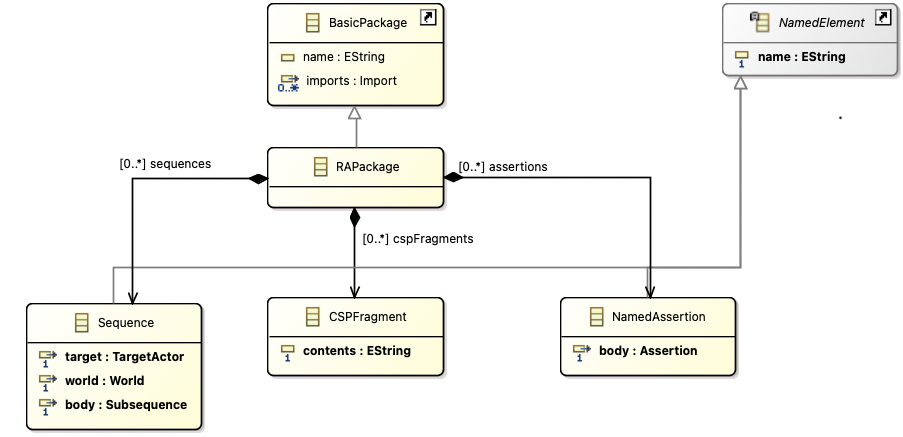
\includegraphics[width=.8\textwidth]{diagrams/top.png}
	\caption{Class diagram for the top of the \langname{} metamodel.}
	\label{fig:metamodel-top}
\end{figure}

\Cref{fig:metamodel-top} is the top-level metamodel diagram for \langname.

Each \langname{} script contains an \mrapackage,\footnote{\mrapackage{} stands
for `RoboStar Assertions package'; we use this name because \mrcpackage{} is
already used for RoboChart packages.}
which is a type of RoboStar \mbasicpackage.
Each \mrapackage{} can contain zero or more of each of these types of content:

\begin{itemize}
\item
	\msequence{}
	(\cref{sec:metamodel-sequences}):
	a sequence diagram;
\item
	\mcspfragment:
	a CSP fragment, currently not bound to a particular process
	\todo{this will change};
\item
	\mnamedassertion{}
	(\cref{sec:metamodel-assertions}):
	a named assertion, currently over sequence diagrams only
	\todo{more types of assertion will appear};
\end{itemize}

\todo{Elements might need to inherit from a common class and be stored in
the same list at some point.}


\section{Sequences, subsequences, and steps}\label{sec:metamodel-sequences}

\begin{figure}
	\centering
	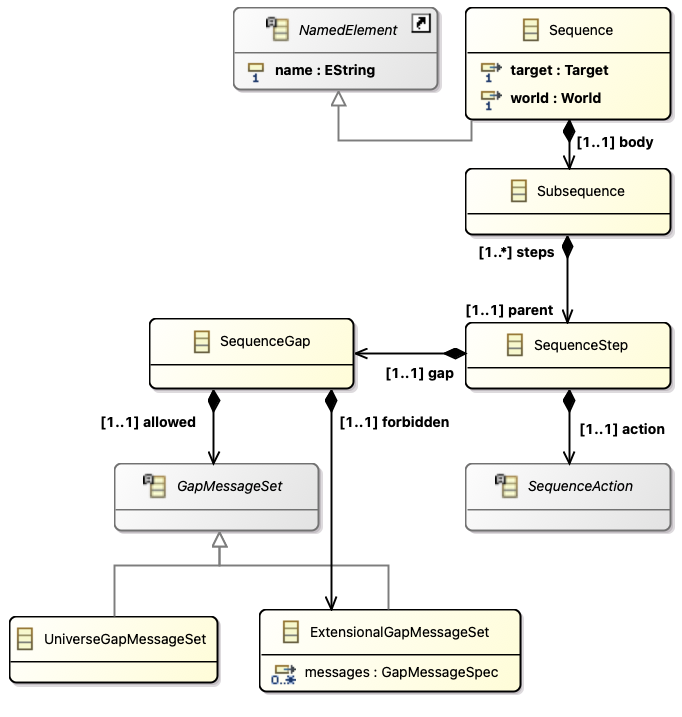
\includegraphics[width=\textwidth]{diagrams/sequences.png}
	\caption{Class diagram for the part of the \langname{} metamodel dealing with sequences.}
	\label{fig:metamodel-sequences}
\end{figure}

\Cref{fig:metamodel-sequences} depicts the part of the metamodel concerning
sequence diagrams.

\subsection{Sequences}

\begin{lstlisting}[style=Example]
sequence Example
  for module ModuleName as M,  // target actor (RoboChart module)
      world             as W   // world actor
{
	anything until end  // subsequence
}
\end{lstlisting}

A \msequence{} represents a single sequence diagram.  It is a \mnamedelement{}
that contains:

\begin{itemize}
\item
	a \msubsequence{} (\cref{ssec:metamodel-sequences-subsequences})
	containing the body of the diagram;
\item
	two \mactor s (\cref{sec:metamodel-actors}):
	a \mtargetactor{} (\cref{ssec:metamodel-actors-target})
	and a \mworld{} (\cref{ssec:metamodel-actors-world}).
\end{itemize}

\subsection{Subsequences}\label{ssec:metamodel-sequences-subsequences}

\begin{lstlisting}[style=Example]
{
	anything until operation O1() from M to W  // step
then
	operation O2() from M to W                 // step
then
	end                                        // step
}
\end{lstlisting}

A \msubsequence{} is a sequential composition of one or more \msequencestep s
(\cref{ssec:metamodel-sequences-steps}).
All \msequence s contain at least one \msubsequence{} at the top level, but
may contain multiple nested \msubsequence s introduced by constructs such as
\mloopaction s.

\subsection{Steps}\label{ssec:metamodel-sequences-steps}

\begin{lstlisting}[style=Example]
anything until             // gap
operation O() from M to W  // action
\end{lstlisting}

A \msequencestep{} is a single step in a \msubsequence.  It consists of a
\msequencegap{} (\cref{ssec:metamodel-sequences-gaps}) and a
\msequenceaction{} (\cref{sec:metamodel-sequences-actions}).

\subsection{Gaps}\label{ssec:metamodel-sequences-gaps}

\begin{lstlisting}[style=Example]
anything
	in     { operation O1() from M to W, operation O2() from M to W }  // allow set
	except { operation O2() from M to W }                              // forbid set

	// a universe set is implied for the allow set if 'in {..}' is omitted
	// an empty extensional set is implied for the forbidden set if 'except {..}' is omitted
until // only permits O1
\end{lstlisting}

A \msequencegap{} represents a condition on any communication\footnote{In PSCs,
this would correspond to \emph{intraMSG}s.} that can happen
\emph{before} a \msequenceaction.  
It contains two \mgapmessageset s: one specifying the messages
\emph{allowed} to pass inside the gap, and another specifying the messages
\emph{forbidden} to pass.\footnote{The \emph{forbidden} set is always an
\mextensionalgapmessageset, as any gap with a universal
\emph{forbidden} set would always be equivalent to one with an empty
\emph{allowed} set.
}

\paragraph{Gap message sets}

A \mgapmessageset{} is an expression of the set of messages allowed or forbidden
inside a \msequencegap.  There are two types of \mgapmessageset:

\begin{itemize}
\item
	a \muniversegapmessageset{} represents the universal set containing 
	all possible messages, and
	captures a lack of specific restriction on
	the \emph{allowed} set of a \msequencegap;
\item	
	an \mextensionalgapmessageset{} is a set (expressed as an unordered list) of
	zero or more \mgapmessagespec s, themselves
	a type of \mmessagespec{} (\cref{sec:metamodel-messages}).
\end{itemize}

There is not yet any meaningful extra data stored in
\mgapmessagespec s that is not present in \mmessagespec s, but this is subject
to change.


\subsection{Actions}\label{sec:metamodel-sequences-actions}

\begin{lstlisting}[style=Example]
operation O1() from M to W  // arrow action

loop L {
	operation O2() from M to W
}  // loop action (taking a subsequence)

end  // final action
\end{lstlisting}

A \msequenceaction{} is an explicit communication or control flow construct in a
\msubsequence.  There are currently three types of action: arrow, loop, and
final actions.

\paragraph{Arrow actions}

An \marrowaction\footnote{The name signifies both that the actions resemble
PSC \emph{arrowMSG} specifications, and also that they correspond to arrows in
the graphical syntax.} specifies one communication between \mactor s which is on
the sequence specified by the diagram.  Each \marrowaction{} wraps one
\marrowmessagespec{} (\cref{sec:metamodel-messages})
containing the specification proper.
\todo{Eventually these will bind arguments.}

\paragraph{Loop actions}

A \mloopaction{} is a \emph{named} infinite loop.  \todo{Breaking and perhaps
other forms of loop are forthcoming.}  Each \mloopaction{} contains one
\msubsequence{} of steps to repeat indefinitely.
\todo{If \mloopaction s could contain zero \msubsequence s, or \msubsequence s
could contain zero \msequencestep s, they could
explicitly capture deadlock, but currently so does \mfinalaction.}

\paragraph{Final actions}

A \mfinalaction{} represents the end of a sequence diagram, corresponding
to a point in time where the sequence target has either terminated or stopped
responding.  It primarily serves to allow a final \msequencegap{} to specify
any permitted communications after the behaviour explicitly specified by the
diagram has occurred.
\todo{Is the termination behaviour correct here?  Are there any useful
parallels between this and a hypothetical empty-bodied loop action?}


\section{Message specifications and topics}\label{sec:metamodel-messages}

\begin{figure}
	\centering
	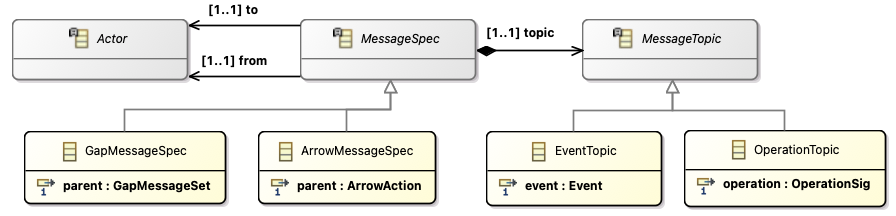
\includegraphics[width=.8\textwidth]{diagrams/messages.png}
	\caption{Class diagram for the part of the \langname{} metamodel dealing with messages.}
	\label{fig:metamodel-messages}
\end{figure}

\Cref{fig:metamodel-messages} depicts the part of the metamodel concerning
message specifications (`specs').

\subsection{Message specifications}

\begin{lstlisting}[style=Example]
operation O1() from M to W  // spec with operation topic, from actor M to actor W
event E        from W to M  // spec with event topic, from actor W to actor M
\end{lstlisting}

A \mmessagespec{} is a specification on the types of communication that can
happen during a gap (a \mgapmessagespec) or arrow (an \marrowmessagespec).\footnote{
This class distinction resembles that in PSCs betweeen intraMSGs and arrowMSGs,
respectively.}  Each \mmessagespec{} contains:

\begin{itemize}
\item
	references to two \mactor s, representing the \emph{to} and \emph{from}
	edges of the communication;
\item
	the \mmessagetopic{} (\cref{ssec:metamodel-messages-topics}) specifying
	the type of communication that the spec is capturing.
\end{itemize}

\subsection{Topics}\label{ssec:metamodel-messages-topics}

A \mmessagetopic{} identifies the specific type of communication in a
\mmessagespec{}.  There are currently two types of topic, corresponding to
RoboChart operations (\moperationmessagetopic) and events (\meventmessagetopic).
Each contains a reference to the signature of the respective construct.
Parameterised operations and events are not yet supported \todo{this will
change soon}.


\section{Actors}\label{sec:metamodel-actors}

\begin{figure}
	\centering
	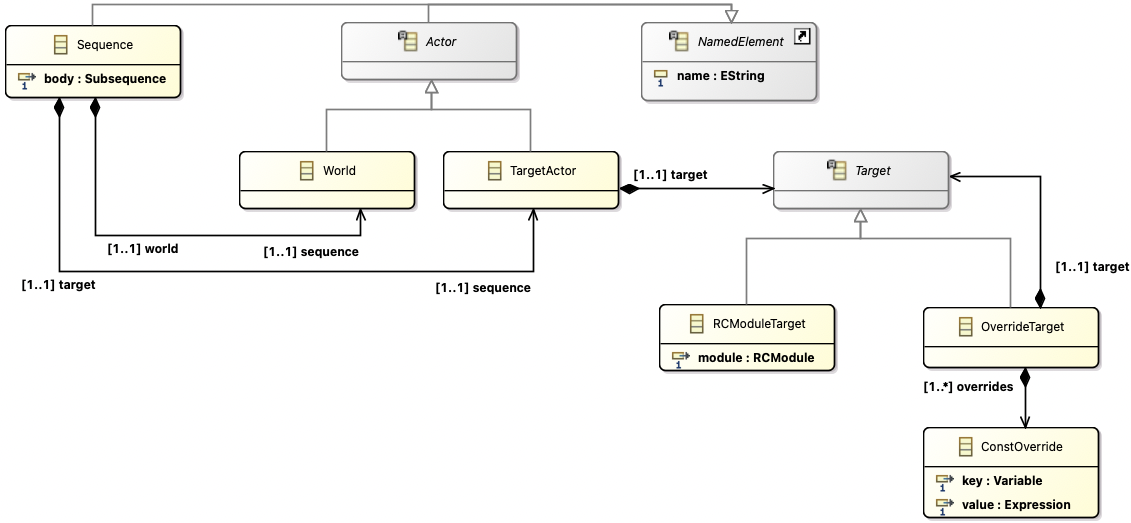
\includegraphics[width=\textwidth]{diagrams/actors.png}
	\caption{Class diagram for the part of the \langname{} metamodel dealing with actors.}
	\label{fig:metamodel-actors}
\end{figure}

\Cref{fig:metamodel-actors} depicts the part of the metamodel concerning
actors.

An \mactor{} is a named participant in a sequence.  The names can be used to
specify the direction of travel in \mmessagespec{}s.
As mentioned in
\cref{sec:metamodel-sequences}, there are always two actors
attached to a sequence: a \mtargetactor{} (\cref{ssec:metamodel-actors-target})
and a \mworld{} (\cref{ssec:metamodel-actors-world}).

\subsection{Targets and target actors}\label{ssec:metamodel-actors-target}

A \mtarget{} is an \emph{anonymous} specification of the part of a robotic
system that serves as the focus for a particular sequence diagram.  There are
presently two types of target, with more to appear later:

\begin{itemize}
\item
	a \mrcmoduletarget{} references a \mrcmodule;
\item
	an \moverridetarget{} wraps another \mtarget, overriding constant
	definitions.
\end{itemize}

A \mtargetactor{} wraps a \mtarget{} with a name, making it suitable as an
\mactor.  The separation between \mtarget{} and \mtargetactor{} allows for
patterns like \moverridetarget{} to exist without introducing unnecessary names.

\subsection{Worlds}\label{ssec:metamodel-actors-world}

A \mworld{} is an \mactor{} that represents the `world' outside a sequence
diagram's target.  \mworld s do not contain any data.

\section{Assertions}\label{sec:metamodel-assertions}

\begin{figure}
	\centering
	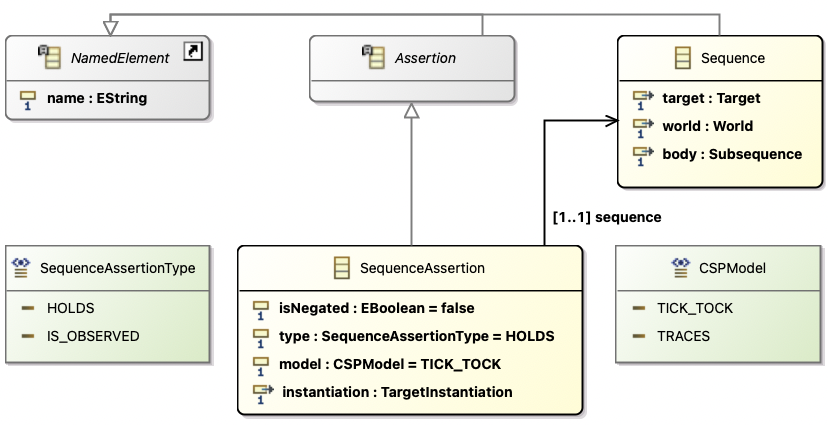
\includegraphics[width=0.7\textwidth]{diagrams/assertions.png}
	\caption{Class diagram for the part of the \langname{} metamodel dealing with assertions.}
	\label{fig:metamodel-assertions}
\end{figure}

\Cref{fig:metamodel-assertions} depicts the part of the metamodel concerning
assertions.

An \massertion{} is an \emph{anonymous} assertion statement.  Currently, there is
only one type of assertion: a \msequenceassertion{}.  \todo{This will change
when merging with the existing language, if not sooner.}

A \msequenceassertion{} is an assertion about a particular \msequence{} with
respect to a particular \mtarget.  By default, the \mtarget{} is that of the
\msequence{}. \todo{This isn't yet explicit in the metamodel.}  Specifying a
custom \mtarget{} as part of the assertion instead makes the assertion refer
to that target.

The specific sequence assertion type comes from the \msequenceassertiontype:
either `sequence holds on target' (refinement), or `sequence is observed on
target' (reverse refinement).  The assertion can be negated.  The choice of
\mcspmodel{} affects how the assertion is checked with CSP tools such as FDR
\todo{the models are incorrect in respect to timed assertions; I haven't yet
decided the best approach to allow the appropriate models in both timed and
untimed modes.  Currently, everything is untimed, and this too will change.}

A \mnamedassertion{} binds an \massertion{} to a name.


\chapter{Semantics}
%!TEX root=./robocert.tex

% Target language colouration
\newcommand{\tlang}[1]{\textcolor{TColor}{\boxed{#1}}}
% Object language colouration (nested inside target language)
\newcommand{\olang}[1]{\boxed{\textcolor{ZedColor}{#1}}}

\newcommand{\tockcsp}{\emph{tock}-CSP}
\newcommand{\cspm}{CSP\(_\text{M}\)}

\newcommand{\defeq}{\mathbin{\overset{\text{def}}=}}
% CSP operators
\newcommand{\interrupt}{\mathbin{\triangle}}
\newcommand{\cspnsop}{\mathbin{\!:\!:\!}}
% CSP keywords/processes
\newcommand{\cspkw}[1]{\operatorname{\mathbf{#1}}}
\newcommand{\runproc}[1]{\cspkw{Run}\left(#1\right)}
\newcommand{\events}{\cspkw{Events}}

%
% Metasyntactic variables
%
\newcommand{\acontext}{c}
\newcommand{\anexpr}{e}
\newcommand{\avar}{v}
% Top-level
\newcommand{\apkg}{P}
\newcommand{\acsp}{f}
% Sequences
\newcommand{\aseq}{\sigma}
\newcommand{\asseq}{q}
\newcommand{\astep}{s}
\newcommand{\agap}{g}
% Actions
\newcommand{\anaction}{a}
\newcommand{\anarrow}{\rho}
\newcommand{\aloop}{l}
% Messages
\newcommand{\amspec}{m}
\newcommand{\amsgset}{M}
\newcommand{\aumsgset}{\amsgset_{\universe}}
\newcommand{\anemsgset}{\amsgset_{e}}
\newcommand{\armsgset}{\amsgset_{r}}
\newcommand{\anevent}{\epsilon}
\newcommand{\anop}{o}
% - Arguments
\newcommand{\anarg}{x}
\newcommand{\anexprarg}{\anarg_\anexpr}
\newcommand{\arestarg}{\anarg_r}
\newcommand{\anarglist}{\mathbf{x}}
% Actors
\newcommand{\atarget}{t}
\newcommand{\aninst}{\phi}
\newcommand{\aworld}{w}
% Assertions
\newcommand{\anasst}{\alpha}
\newcommand{\asasst}{\alpha_s}
\newcommand{\amodel}{\mathcal{M}}

% External semantics
\newcommand{\exprsema}[2]{\sema{#1}{expr}_{(#2)}}

\newcommand{\sema}[2]{\llbracket #1 \rrbracket^{\mathsf{#2}}}
\newcommand{\pkgsema}[1]{\sema{#1}{pkg}}
\newcommand{\cspsema}[1]{\sema{#1}{csp}}
\newcommand{\stepsema}[1]{\sema{#1}{step}}
\newcommand{\gapsema}[2]{\sema{#1}{gap}_{(#2)}}
\newcommand{\actsema}[1]{\sema{#1}{act}}
\newcommand{\mspecsema}[2]{\sema{#1}{mspec}_{\text{#2}}}
\newcommand{\pmspecsema}[1]{\mspecsema{#1}{prefix}}
\newcommand{\emspecsema}[1]{\mspecsema{#1}{events}}
\newcommand{\arglistsema}[2]{\sema{#1}{args}_{(#2)}}
\newcommand{\loopsema}[1]{\sema{#1}{loop}}
\newcommand{\msgsetsema}[1]{\sema{#1}{mset}}
\newcommand{\seqsema}[1]{\sema{#1}{seq}}
\newcommand{\sseqsema}[1]{\sema{#1}{sseq}}
\newcommand{\asstsema}[1]{\sema{#1}{asst}}

\newcommand{\targetsema}[2]{\sema{#1}{target}_{(#2)}}

\newcommand{\funcname}[1]{\ensuremath{\mathsf{#1}}}
\newcommand{\eventsOf}[1]{\funcname{events}(#1)}
\newcommand{\seqnameOf}[1]{\funcname{seqName}(#1)}
\newcommand{\ctargetnameOf}[1]{\funcname{ctargetName}(#1)}
\newcommand{\otargetnameOf}[1]{\funcname{otargetName}(#1)}

\newcommand{\field}[2]{#1.\funcname{#2}}

This chapter formally captures the semantics of \langname{} in terms of its
target languages:

\begin{itemize}
\item
	\tockcsp~(\cref{sec:semantics-tockcsp});
\item
	\todo{PRISM};
\item
	\todo{Isabelle/UTP?}.
\end{itemize}

Each semantics captures \massertion s as the top-level definition, with all
objects reachable from the assertions translated in-line.  As a
consequence, we do not capture organisational details such as \mrapackage s,
or any distinction between references to objects and their definitions.

\section{How to read this section}

\begin{table}
  \centering

  \begin{tabular}{p{2em}p{10.5em}}
    \toprule
    \thead{Var.}
    & \thead{Type}
    \\
    \midrule
    \multicolumn{2}{l}{\tsubhead{\robochart{} imports}}
    \\
    \(\avar\) & \mvariable
    \\
    \(\anexpr\) & \mexpression
    \\
    \bottomrule
  \end{tabular}
  \begin{tabular}{p{2em}p{10.5em}}
    \toprule
    \thead{Var.}
    & \thead{Type}
    \\
    \midrule
    \multicolumn{2}{l}{\tsubhead{Packages (\cref{sec:metamodel-top})}}
    \\
    \(\apkg\) & \mrapackage
    \\
    \(\acsp\) & \mcspfragment
    \\
    \midrule
    \multicolumn{2}{l}{\tsubhead{Sequences (\cref{sec:metamodel-sequences})}}
    \\
    \(\aseq\) & \msequence
    \\
    \(\asseq\) & \msubsequence
    \\
    \(\astep\) & \msequencestep
    \\
    \(\agap\) & \msequencegap
    \\
    \midrule
    \multicolumn{2}{l}{\tsubhead{Steps (\cref{sec:metamodel-steps})}}
    \\
    \(\aloop\) & \mloopstep
    \\
    \midrule
    \multicolumn{2}{l}{\tsubhead{Actions (\cref{sec:metamodel-actions})}}
    \\
    \(\anaction\) & \msequenceaction
    \\
    \(\anarrow\) & \marrowaction
    \\
    \(\bot\) & \mfinalaction
    \\
    \\
    \\
    \\
    \\
    \bottomrule
  \end{tabular}
  \begin{tabular}{p{2em}p{10.5em}}
    \toprule
    \thead{Var.}
    & \thead{Type}
    \\
    \midrule
    \multicolumn{2}{l}{\tsubhead{Messages (\cref{sec:metamodel-messages})}}
    \\
    \(\amspec\) & \mmessagespec
    \\
    \(\amsgset\) & \mmessageset
    \\
    \(\aumsgset\) & \muniversemessageset
    \\
    \(\anemsgset\) & \mextensionalmessageset
    \\
    \(\armsgset\) & \mrefmessageset
    \\
    \(\anarg\) & \margument
    \\
    \(\anexprarg\) & \mexpressionargument
    \\
    \(\arestarg\) & \mrestargument
    \\
    \midrule
    \multicolumn{2}{l}{\tsubhead{Actors (\cref{sec:metamodel-actors})}}
    \\
    \(\atarget\) & \mtarget
    \\
    \(\aworld\) & \mworld
    \\
    \(\aninst\) & \mtargetinstantiation
    \\
    \midrule
    \multicolumn{2}{l}{\tsubhead{Assertions (\cref{sec:metamodel-assertions})}}
    \\
    \(\anasst\) & \massertion
    \\
    \(\asasst\) & \msequenceassertion
    \\
    \(\amodel\) & \mcspmodel	
    \\
    \bottomrule
  \end{tabular}
  
  \caption{Metasyntactic variables.}
  \label{tab:metasyntactic-variables}
\end{table}

The semantics treatments in this section take the form of rewrite rules from
the abstract syntax in \cref{cha:metamodel} to some object language (for
instance, \tockcsp).
For conciseness, we use a meta-language based on the Z notation.
We also use the following notational conventions:

\begin{itemize}
\item
	\(\sema{-}{name}\) denotes a main semantic rule;
\item
	\(\funcname{name}()\) denotes auxiliary semantic functions;
\item
	\(\field{x}{name}\) denotes a field of the metamodel object \(x\);
\item
	\tlang{\text{boxed shaded text}} denotes a construct from the object
	language; outside such text, or \tlang{\olang{\text{inside nested boxes}}},
	assume use of the meta-language.  For example, consider the \tockcsp{}
	construct:
	\[\tlang{
		\runproc{\olang{\gapsema{\field{\astep}{gap}}{\field{\astep}{action}}}}
		\interrupt \olang{\actsema{\field{\astep}{action}}}
	}\]
	Here, \(\runproc{}\) and \(\interrupt\) are part of \tockcsp, while
	\(\actsema{\field{\astep}{action}}\) is an semantic operation on the
	\langname{} metamodel.
\item
	variables in the meta-language have an implicit metamodel type
	corresponding to one of the metasyntactic variables in
	\cref{tab:metasyntactic-variables}.
\end{itemize}

\section{Dependencies on the \robochart{} semantics}

\newcommand{\targetProcess}[1]{\ensuremath{\funcname{targetProcess}\left(#1\right)}}
\newcommand{\targetParams}[1]{\ensuremath{\funcname{targetParams}\left(#1\right)}}
\newcommand{\constName}[1]{\ensuremath{\funcname{constName}\left(#1\right)}}

\todo{this may need to move to the \tockcsp{} section eventually}

Each semantics treatment in this section assumes the existence of a compatible
semantics over \robochart.  Specifically, we assume the following rules and
functions are available, or can be derived, from such a semantics:

\begin{itemize}
\item
	let \targetProcess{-} map a target to the parametric
	process exposed by the relevant \tockcsp{} semantics (for instance,
	we delegate to the \robochart{} semantics for the underlying
	\mrcmodule{} of a \mrcmoduletarget);
	\todo{doesn't account for the ID parameter in certain target
	processes};
\item
	let \targetParams{-} map a target to the sequence of
	constants in its parameterisation;
\item
	let \constName{-} map a constant to its name in the \robochart{}
	instantiations file;
\item
	let \(\exprsema{\anexpr}{\acontext}\) be the expression semantics of 
	\(\anexpr\) in the context \(\acontext\).  The expression semantics
	is external to this semantics, but is largely that of Z.
\end{itemize}

\section{\tockcsp{} semantics}\label{sec:semantics-tockcsp}
%!TEX root=../robocert.tex

This section introduces a \tockcsp{} semantics for \langname.
\todo{Need to make sure it's actually \tockcsp, not CSP.}
This semantics is inspired by that of Lima et al. on the CML semantics of
UML sequence diagrams.

The behaviour of the \langname{} generator is expected to conform to
this semantics, except that:

\begin{itemize}
\item
  The generator targets \cspm{} instead of CSP, and so \emph{may}
  use semantically equivalent \cspm{} constructs where the CSP equivalents
  are missing or not idiomatic;
\item
  The generator \emph{must} \todo{not yet but eventually} wrap processes in
  timed sections and prioritisations to achieve the appropriate \tockcsp{} behaviours of
  CSP operators;
\item
  The generator \emph{may} perform semantics-preserving optimisations,
  such as substituting \(P\) for \(\tlang{\Stop \interrupt \olang{P}}\).
\end{itemize}

\todo{Some of the definitions are very loosely typed (as they are expanding from
a metamodel to textual snippets of something halfway between \tockcsp{} and
\cspm), and it'd be nice to fix that and/or give explicit result types.}

\subsection{Assertions}

The definitions here correspond to \cref{sec:metamodel-assertions}.

\begin{definition}[\massertion]

\newcommand{\refop}[3]{\mathbin{\odot_{#1}^{(#2, #3)}}}

The only type of assertion so far is \msequenceassertion.  The semantics of a
\msequenceassertion{} relates the \msequence{} of the assertion to the
\mtarget{} of the assertion.
%
\begin{align*}
	\asstsema{\asasst}
\quad\defeq\quad&
	\seqnameOf{\field{\asasst}{sequence}}
	\;
	\refop{\field{\asasst}{model}}{\field{\asasst}{isNegated}}{\field{\asasst}{type}}
	\;
	\targetsema{\field{\field{\asasst}{sequence}}{target}}{\field{\asasst}{instantiation}}
\end{align*}

The exact refinement operator depends on the assertion type and negation:
%
\begin{align*}
	\refop{\amodel}{\true}{\mathsf{holds}}
\quad\defeq\quad&
	\tlang{\sqsubseteq_{\olang{\amodel}}}
&
	\refop{\amodel}{\false}{\mathsf{holds}}
\quad\defeq\quad&
	\tlang{\not\sqsubseteq_{\olang{\amodel}}}
\\
	\refop{\amodel}{\true}{\mathsf{isObserved}}
\quad\defeq\quad&
	\tlang{\sqsupseteq_{\olang{\amodel}}}
&
	\refop{\amodel}{\false}{\mathsf{isObserved}}
\quad\defeq\quad&
	\tlang{\not\sqsupseteq_{\olang{\amodel}}}
\\
\end{align*}
\end{definition}


\subsection{Sequences}\label{ssec:semantics-tockcsp-sequences}

The definitions here correspond to \cref{sec:metamodel-sequences}.

\begin{definition}[\msequence]

The semantics of a \msequence{} is that of its subsequence
\todo{eventually, in parallel with its memory}.
%
\begin{align*}
	\seqsema{\aseq}
\quad\defeq\quad&	
	\sseqsema{\field{\aseq}{body}}
\end{align*}

\end{definition}

\begin{definition}[\msubsequence]

The semantics of a \msubsequence{} is a sequential composition of that of its steps.
%
\begin{align*}
	\sseqsema{\asseq}
	\quad\defeq\quad&	
	\funcname{steps}(\field{\asseq}{body})
\\
	\funcname{steps}(\langle \astep_1, \dotsc, \astep_n \rangle)
	\quad\defeq\quad&	
	\tlang{
	\olang{\stepsema{\astep_1}}
	\circseq
	\olang{\dotso}
	\circseq
	\olang{\stepsema{\astep_n}}
	}
\end{align*}

\end{definition}

\todo{\msequencestep}

\begin{definition}[\mactionstep]

The semantics of a \mactionstep{} is an unbounded loop over the events of its
\msequencegap, interrupted by the \msequenceaction.\footnote{Note that the semantics of the gap depends
on the action.  This is because, as seen in \(\gapsema{\agap}{\anaction}\),
the events on which the action can interrupt the
gap must be removed from the events of the gap to ensure the interrupt has the
expected semantics.}
%
\begin{align*}
	\stepsema{\astep}
\quad\defeq\quad&	
	\tlang{
		\runproc{\olang{\gapsema{\field{\astep}{gap}}{\field{\astep}{action}}}}
		\interrupt \olang{\actsema{\field{\astep}{action}}}
	}
\end{align*}
\end{definition}

\begin{definition}[\msequencegap]
	The semantics of a \msequencegap{} is the CSP event set corresponding to
	the difference between the \emph{allowed} set and any events
	the action following the gap can initially communicate.
%
\begin{align*}
	\gapsema{
		\agap
	}{\anaction}
\quad\defeq\quad&
\tlang{
	\olang{\msgsetsema{\field{\agap}{allowed}}}
	\setminus
	\olang{\eventsOf{\anaction}}
}
\end{align*}
\end{definition}

\begin{definition}[CSP event sets]
For now, the event set of an action is the prefix of an arrow action, or
the empty set for any other actions.  This will change when the prefix becomes
inexpressible as an event set.
%
\begin{align*}
	\eventsOf{\anarrow}
\quad\defeq\quad&
	\tlang{\Set{\olang{\emspecsema{\anarrow}}}}
	\tag{arrow}
\\
	\eventsOf{\anaction}
\quad\defeq\quad&
	\tlang{\emptyset}
	\tag{anything else}
\end{align*}
\end{definition}

\subsection{Actions}\label{ssec:semantics-tockcsp-actions}

The definitions here correspond to \cref{sec:metamodel-actions}.

\begin{definition}[\msequenceaction]

The semantics of an arrow action is the semantics of its arrow as a CSP prefix,
prefixing termination.  The semantics of a loop delegates to a separate rule
over its label and subsequence.
%
\begin{align*}
	\actsema{\anarrow}
\quad\defeq\quad&
	\tlang{
	\left(
	\olang{\pmspecsema{\anarrow}}
	\then
	\Skip
	\right)
	}
	\tag{arrow action}
\\
	\actsema{\aloop}
\quad\defeq\quad&
	\loopsema{\aloop}
\tag{loop action}
\\
	\actsema{\bot}
\quad\defeq\quad&
	\tlang{\Skip}
\tag{final action}
\end{align*}

\end{definition}

\newcommand{\iloop}[1]{\text{Loop}(#1)}
\newcommand{\nloop}[1]{\text{Loop}_\sqcap(#1)}
\newcommand{\dloop}[2]{\text{Loop}_d(#1, #2)}
\newcommand{\lloop}[2]{\text{Loop}_l(#1, #2)}
\newcommand{\uloop}[2]{\text{Loop}_u(#1, #2)}
\newcommand{\rloop}[3]{\text{Loop}_r(#1, #2, #3)}

\begin{definition}[\mloopstep]  
For now, the semantics of a loop is that of the loop
subsequence hoisted into an auxiliary loop-running process (defined
below).
\todo{define the symbols used here}
%
\begin{align*}
  \loopsema{\aloop}
  \quad\defeq\quad
  &
    \funcname{runner}(\field{\aloop}{bound}, \sseqsema{\field{\aloop}{body}})
  \\
  \funcname{runner}(\infty, P)
  \quad\defeq\quad
  & \tlang{\iloop{\olang{P}}}
    \tag{infinite loops}
  \\
  \funcname{runner}(n, P)
  \quad\defeq\quad
  & \tlang{\dloop{\olang{\exprsema{n}{\emptyset}}}{\olang{P}}}
    \tag{definite-bound loops}
  \\
  \funcname{runner}((l, \ast), P)
  \quad\defeq\quad
  & \tlang{\lloop{\olang{\exprsema{l}{\emptyset}}}{\olang{P}}}
    \tag{lower-bound loops}
  \\
  \funcname{runner}((l, u), P)
  \quad\defeq\quad
  & \tlang{\rloop{\olang{\exprsema{l}{\emptyset}}}{\olang{\exprsema{u}{\emptyset}}}{\olang{P}}}
    \tag{range-bound loops}
  \\  
\end{align*}

\end{definition}

\begin{definition}[Auxiliary loop processes]

We can define the loop processes used above in CSP as follows:
%
\begin{align*}
  \iloop{P}
  \quad\defeq\quad
  & P \circseq \iloop{P}
    \tag{infinite}
  \\
  \nloop{P}
  \quad\defeq\quad
  & \Skip \sqcap \left(P \circseq \nloop{P}\right)
    \tag{nondeterministic}
  \\  
  \dloop{n}{P}
  \quad\defeq\quad
  & \Skip \triangleleft n \leq 0 \triangleright \left(P \circseq \dloop{n-1}{P}\right)
    \tag{definite}
  \\
  \uloop{n}{P}
  \quad\defeq\quad
  & \Skip \triangleleft n \leq 0 \triangleright \left(\Skip \sqcap \left(P \circseq \uloop{n-1}{P}\right)\right)
    \tag{upper-bound}
  \\
  \lloop{n}{P}
  \quad\defeq\quad
  & \dloop{n}{P} \circseq \nloop{P}
    \tag{lower-bound}
  \\
  \rloop{l}{u}{P}
  \quad\defeq\quad
  & \lloop{l}{P} \circseq \uloop{u - l}{P}
    \tag{range}
  \\
\end{align*}
\end{definition}

\subsection{Messages}\label{ssec:semantics-tockcsp-messages}

The definitions here correspond to \cref{sec:metamodel-messages}.

\begin{definition}[\mmessageset]

  The semantics of a message set is the universal event set for \muniversemessageset s;
  the expansion of the given \mgapmessagespec s for \mextensionalmessageset s;
  the semantics of the referred-to set for \mrefmessageset s;
  and the semantics of the referred-to set operator for \mbinarymessageset s.
%
\begin{align*}
  \msgsetsema{\aumsgset}
  \quad\defeq\quad
  &
    \tlang{\events}
    \tag{universe}
  \\
  \intertext{\todo{The meta/object language distinction is messy here
  and I'm not sure how to handle it.}}
  \msgsetsema{\anemsgset}
  \quad\defeq\quad
  &
    \tlang{
    \bigcup
    \olang{
    \Set{
    \emspecsema{\amspec} | \amspec \in \field{\anemsgset}{messages}
    }
    }
    }
    \tag{extensional}
  \\
  \msgsetsema{\armsgset}
  \quad\defeq\quad
  &
    \msgsetsema{\field{\field{\armsgset}{set}}{set}}
    \tag{reference}
  \\
  \msgsetsema{\amsgset_l \odot \amsgset_r}
  \quad\defeq\quad
  &
  \tlang{
    \olang{\msgsetsema{\amsgset_l}}
    \odot
    \olang{\msgsetsema{\amsgset_r}}
    \tag{binary-operator}
  }
\end{align*}
\end{definition}

There are two distinct semantic rules for \mmessagespec s.  One is used whenever
we expand the \mmessagespec{} into an event set, and handles `rest' arguments
by implicitly quantifying over the missing parameters.  The other is used when
expanding to a prefix, and introduces explicit discards for the missing
parameters.  \todo{The two forms will diverge further when we introduce
parameter binding.}

\begin{definition}[\mmessagespec{} as an event set]

We expand \mmessagespec s into event-set form in two stages: expanding
any non-`rest' arguments with \funcname{withArgs}, then expanding the channel
reference using \funcname{msgChan}.
%
\begin{align*}
	\emspecsema{\amspec}
\quad\defeq\quad&
\funcname{withArgs}\left(\field{\amspec}{arguments}, \amspec\right)
\\
	\funcname{withArgs}\left(\amspec, \anarglist\cat\langle\anexprarg\rangle\right)
\quad\defeq\quad&
\tlang{
	\olang{\funcname{withArgs}\left(\amspec, \anarglist\right)}
	!\olang{\exprsema{\anexprarg}{\amspec}}
}
\tag{expression argument}
\\
	\funcname{withArgs}\left(\amspec, \anarglist\cat\langle\arestarg\rangle\right)
\quad\defeq\quad&
	\funcname{withArgs}\left(\amspec, \anarglist\right)
\tag{rest argument}
\\
	\funcname{withArgs}\left(\amspec, \langle\rangle\right)
\quad\defeq\quad&
	\funcname{msgChan}\left(\amspec\right)
\tag{end of arguments}
\end{align*}
The expansion of the message channel
depends on the message topic
and, for certain topics, the direction (inbound from world to target, or
outbound from target to world).
\newcommand{\nsOf}[1]{\mathsf{ns}(#1)}
\newcommand{\targetOf}[2]{\mathsf{target}(#1,#2)}
\newcommand{\topicOf}[3]{\mathsf{topic}(#1,#2,#3)}
%
\begin{align*}
	\funcname{msgChan}(\amspec)
\quad\defeq\quad&
\tlang{
	\olang{\nsOf{\targetOf{\field{\amspec}{from}}{\field{\amspec}{to}}}}
	{}\cspnsop{}
	\olang{\topicOf{\field{\amspec}{topic}}{\field{\amspec}{from}}{\field{\amspec}{to}}}
}
\\
	\targetOf{\aworld}{\atarget}
\quad\defeq\quad&
	\targetOf{\atarget}{\aworld}
	\quad\defeq\quad
	\atarget
\\
	\topicOf{\anop}{\atarget}{\aworld}
\quad\defeq\quad&
\tlang{
	\olang{\field{\anop}{name}}\text{Call}
}
\tag{operation; always outbound}
\\
	\topicOf{\anevent}{\aworld}{\atarget}
\quad\defeq\quad&
	\tlang{\olang{\field{\anevent}{name}}\text{.in}}
\tag{inbound event}
\\
	\topicOf{\anevent}{\atarget}{\aworld}
\quad\defeq\quad&
	\tlang{\olang{\field{\anevent}{name}}\text{.out}}
\tag{outbound event}
\end{align*}
\end{definition}

\newcommand{\paramsOf}[1]{\funcname{params}(#1)}
\newcommand{\beforeRest}[1]{\funcname{beforeRest}(#1)}

\begin{definition}[\mmessagespec{} as a prefix]

To expand a \mmessagespec{} into a prefix, we take the event set expansion and
\todo{for now} \emph{pad} it with wildcard inputs for each topic parameter
left unmatched at the point of any \mrestargument.
%
\begin{align*}
	\pmspecsema{\amspec}
\quad\defeq\quad&
	\funcname{pad}\left(\emspecsema{\amspec}, \funcname{padding}(\amspec)\right)
\\
	\funcname{pad}(x, 0)
\quad\defeq\quad&
	x
\tag{base case}
\\
	\funcname{pad}(x, n)
\quad\defeq\quad&
\tlang{
	\olang{\funcname{pad}(x, n-1)}?\_
}
\tag{inductive case}
\\
	\funcname{padding}(\amspec)
\quad\defeq\quad&
	\#(\paramsOf{\field{\amspec}{topic}}) - \beforeRest{\field{\amspec}{arguments}}
\\
	\beforeRest{\langle\rangle}
\quad\defeq\quad&
	0
\tag{base case}
\\
	\beforeRest{\langle \arestarg \rangle \cat \anarglist}
\quad\defeq\quad&
	0
\tag{rest argument}
\\
	\beforeRest{\langle \anarg \rangle \cat \anarglist}
\quad\defeq\quad&
	1 + \beforeRest{\anarglist}
\tag{non-rest argument}
\end{align*}
\end{definition}

\subsection{Actors}\label{ssec:semantics-tockcsp-actors}

The definitions here correspond to \cref{sec:metamodel-actors}.


\begin{definition}[\mtarget]

The semantics of a target is the parametric process generated for that
target by the relevant external semantics, with constant parameters instantiated
as follows:

\begin{itemize}
\item
	if the constant is bound in the assertion's \mtargetinstantiation{}
	(passed to the semantics as \(\aninst\)), use the bound expression; else
\item
	if the constant is bound in the target's \mtargetinstantiation, use
	the bound expression; else
\item
	use the \(\funcname{constName}\) of the constant, under the assumption
	that it will later bind to a fallback instantiation for the constant.
\end{itemize}
%
\begin{align*}
	\targetsema{\atarget}{\aninst}
\quad\defeq\quad&
\tlang{
	\olang{\funcname{targetProcess}(\atarget)}
	\left(
		\olang{\exprsema{-}{\atarget}\ \circ\ \funcname{instantiate}(\aninst)\ \circ\ \funcname{targetParams}(\atarget)}
	\right)
}
\\
	\funcname{instantiate}(\aninst, \atarget)
\quad\defeq\quad&
	\funcname{constName}
	\oplus
	\field{\field{\atarget}{instantiation}}{constants}
	\oplus
	\field{\aninst}{constants}
\end{align*}
\end{definition}


%%% Local Variables:
%%% mode: latex
%%% TeX-master: "../robocert"
%%% End:


%%% Local Variables:
%%% mode: latex
%%% TeX-master: "robocert"
%%% End:


\end{document}